\subsection{Hardware Setup}
Der Raspberry Pi muss mit seiner Stromversorgung (USB C), einem  Netzwerk (Ethernet) und 1-12 Sensorboards verbunden werden.
\subsection{Messung Starten}
Über das Terminal (Unter Windows cmd) muss eine SSH Verbindung zum Raspberry Pi aufgebaut werden.\\
\textbf{ssh pi@[IP-ADRESSE]}\\
Die Messsoftware wurde automatisch in einem Screen mit den Namen SpectralSensor gestartet. Um die Messung zu starten muss sich mit diesem Screen verbunden werden.\\
\textbf{screen -r}\\
\begin{figure}[H]
\centering
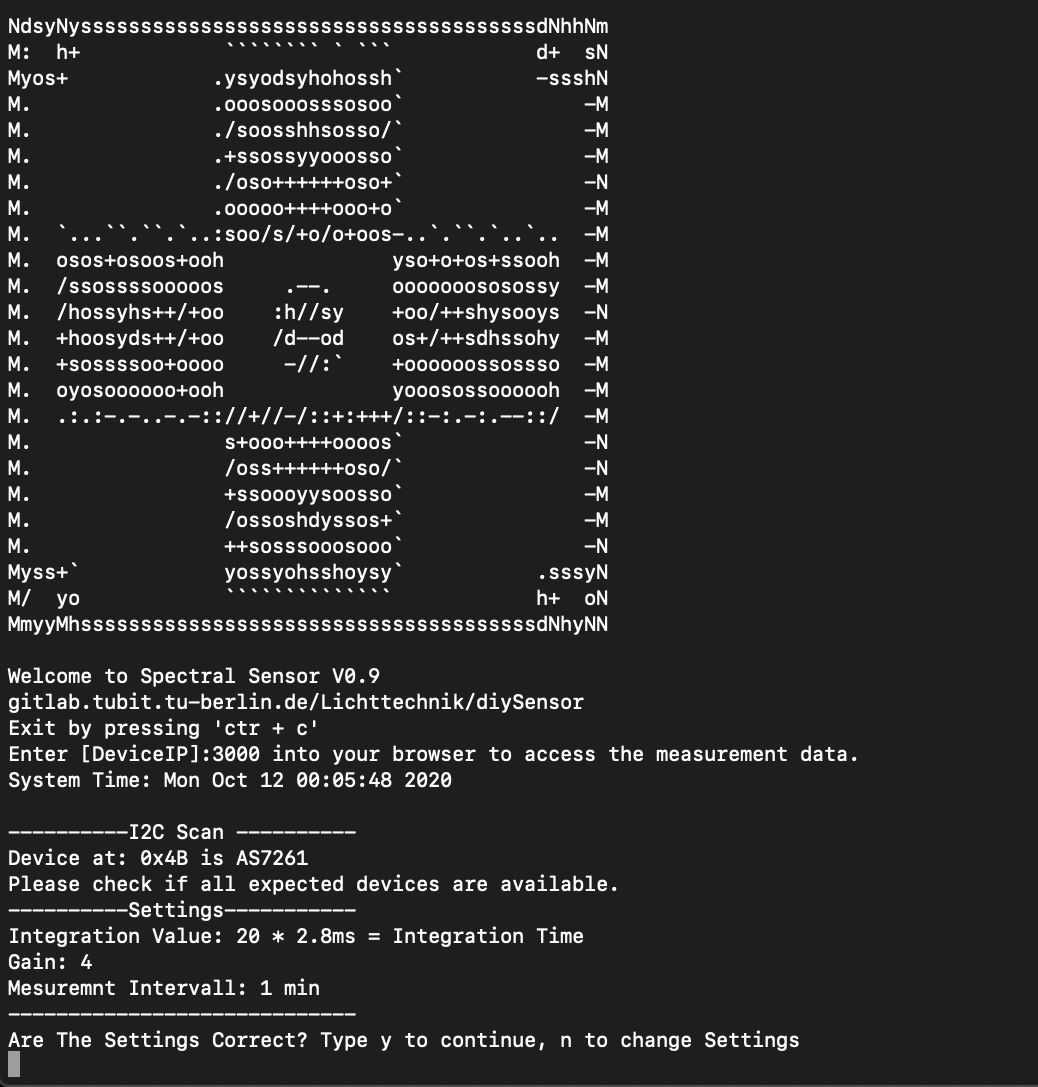
\includegraphics[width=0.7\textwidth]{img/handbuch/check_settings}
\caption{Terminal Output bei Start der Messsoftware }
\label{fig:Start-der-Messsoftware}
\end{figure}
\noindent Zuerst muss im Terminaloutput überprüft werden ob der NTP Server synchronisiert ist.
Wird eine falsche Systemzeit, angezeigt muss das Programm nach etwa 40 Sekunden neu Gestartet werden. Anschließend sollte die Systemzeit richtig sein. (Mehr zum Programm Neustart: \ref{restart}).\\
Im I2C Scann sollten alle angeschlossenen Sensoren angezeigt werden.\\
Die Messung wird mit den angezeigten Einstellungen gestartet, indem die Eingabeaufforderung mit \textbf{Y} bestätigt wird.\\
\begin{figure}[H]
\centering
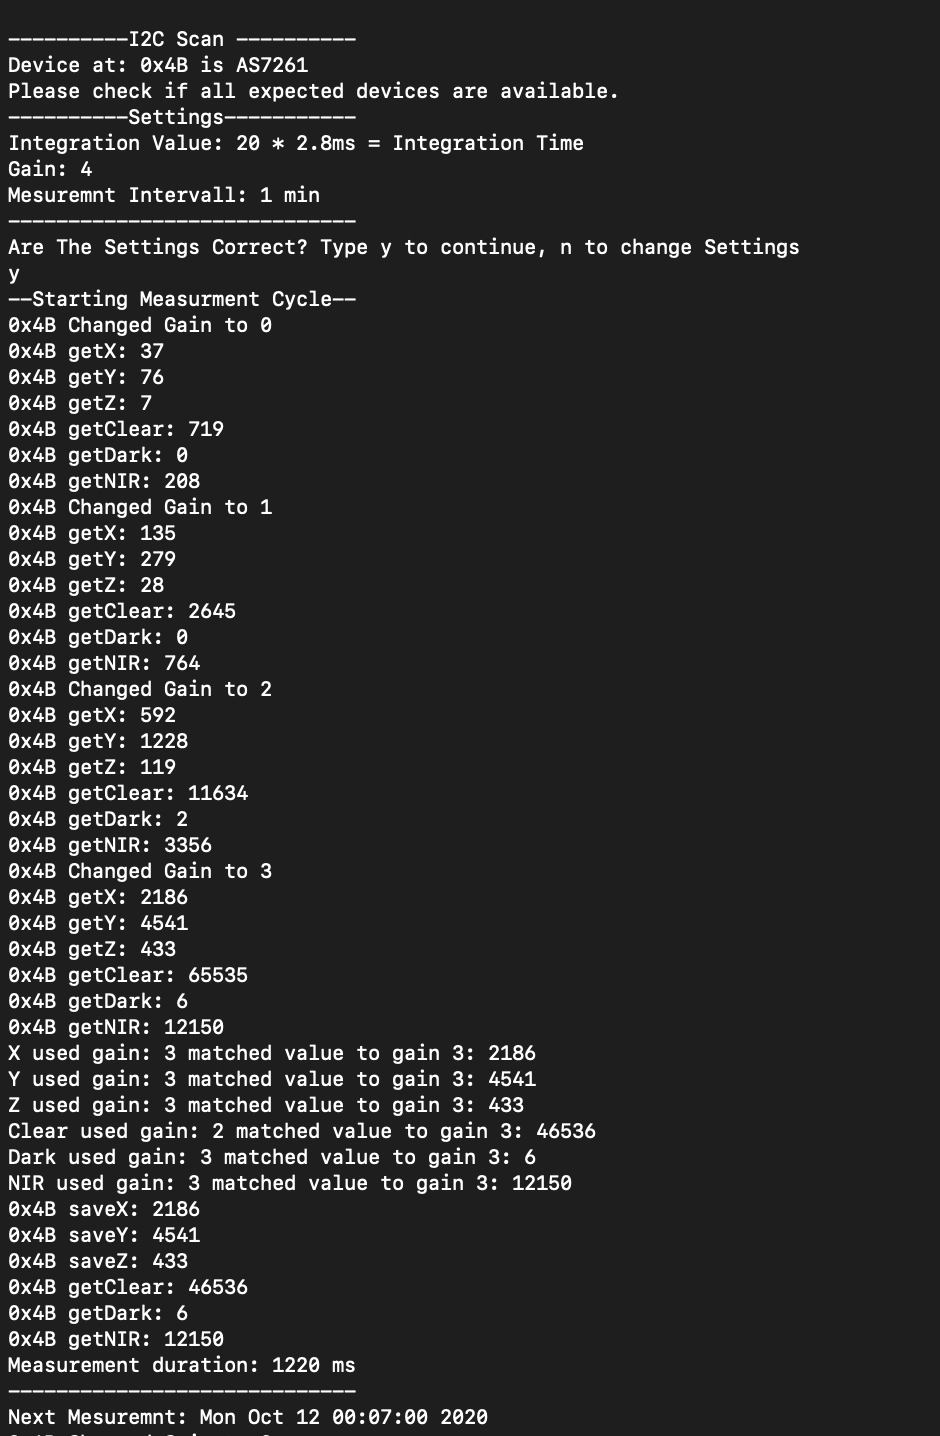
\includegraphics[width=0.7\textwidth]{img/handbuch/y_start_measurement}
\caption{Terminal Output bei Start der Messung }
\label{fig:Start-der-Messung}
\end{figure}

Um die Einstellung zu verändern wird \textbf{N} ausgewählt.\\
\begin{figure}[H]
\centering
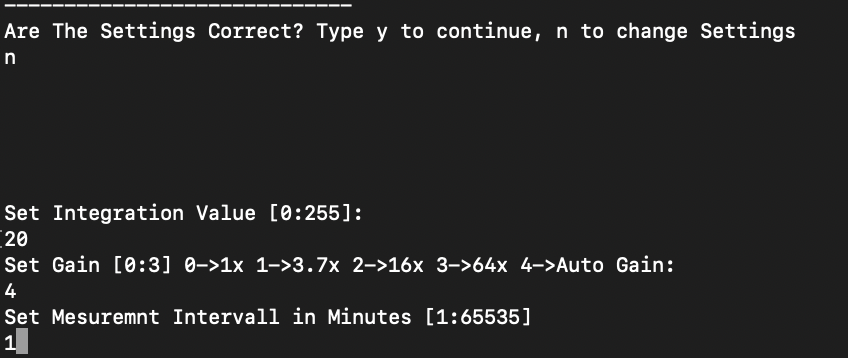
\includegraphics[width=0.7\textwidth]{img/handbuch/n_change_settings}
\caption{Beispielhafter Terminal Output bei Einstellungsänderungen}
\label{fig:changesettings}
\end{figure}
\subsection{Webinterface}
Das Grafana Webinterface ist unter folgender Adresse im Browser zu erreichen:\\
\textbf{[IP-ADRESSE]:3000}

\begin{figure}[H]
\centering
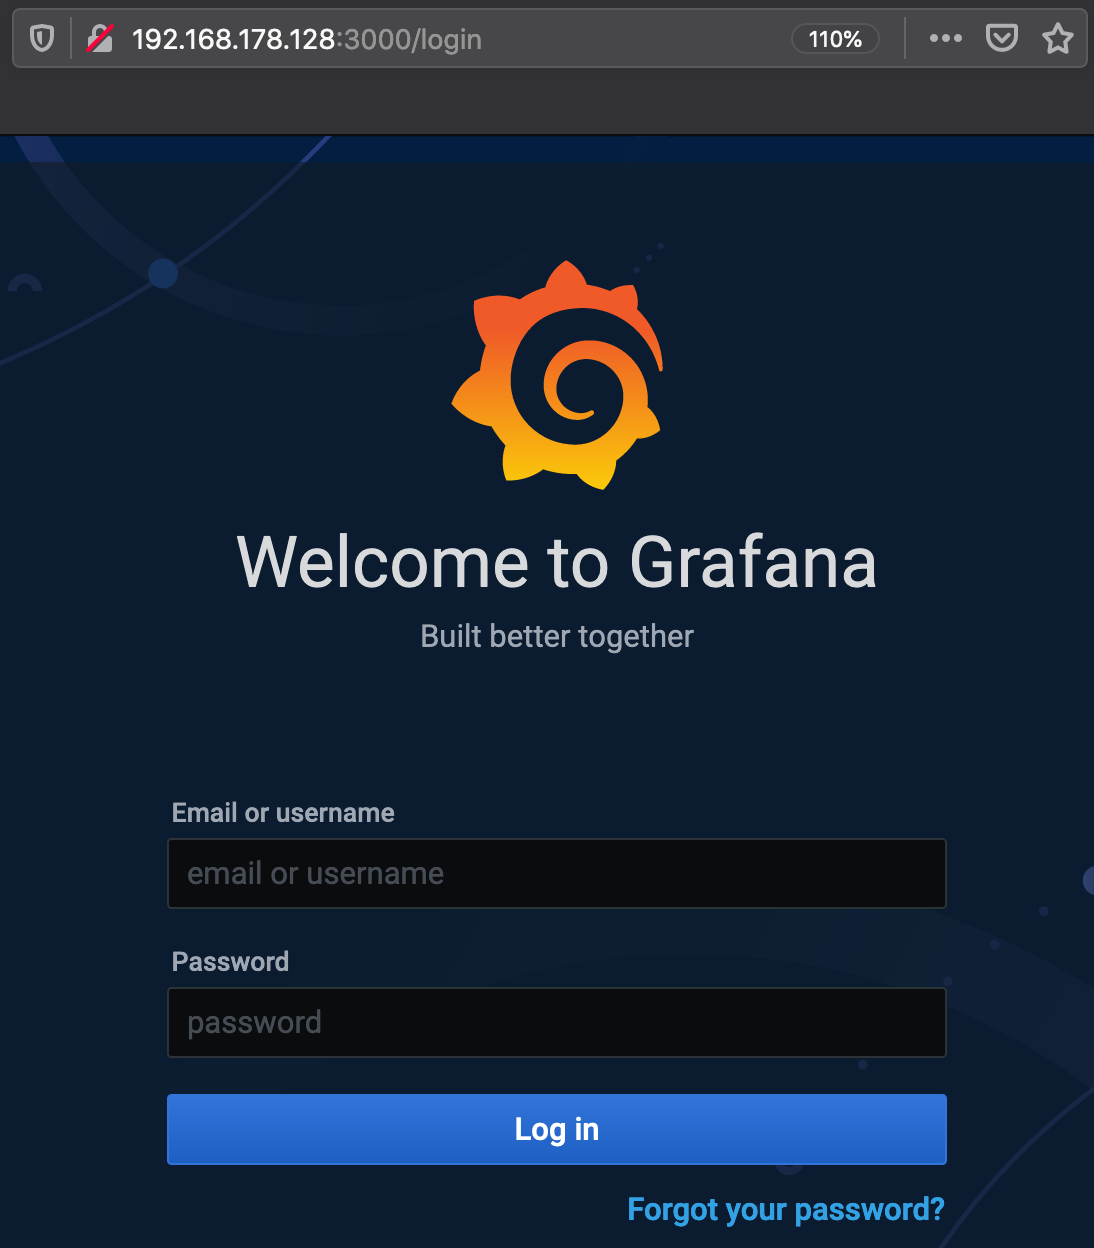
\includegraphics[width=0.6\textwidth]{img/handbuch/grafna_login}
\caption{Grafana Login im Browser}
\label{fig:grafna_login}
\end{figure}
Im Example Dashboard sind alle Sensordatenplots vorhanden. Wenn weniger Plots benötigt werden oder die Darstellung angepasst werden muss, kann eine Kopie angefertigt und bearbeitet werden.\\
Um Daten im CSV-Format zu exportieren muss zuerst der gewünschte Zeitbereich ausgewählt werden.
Anschließend wird, wie in Abbildung \ref{fig:export_data} zu sehen, im Kontextmenü (Klick auf den Namen eines Plots) unter Inspect die Option Data ausgewählt. 

\begin{figure}[H]
\centering
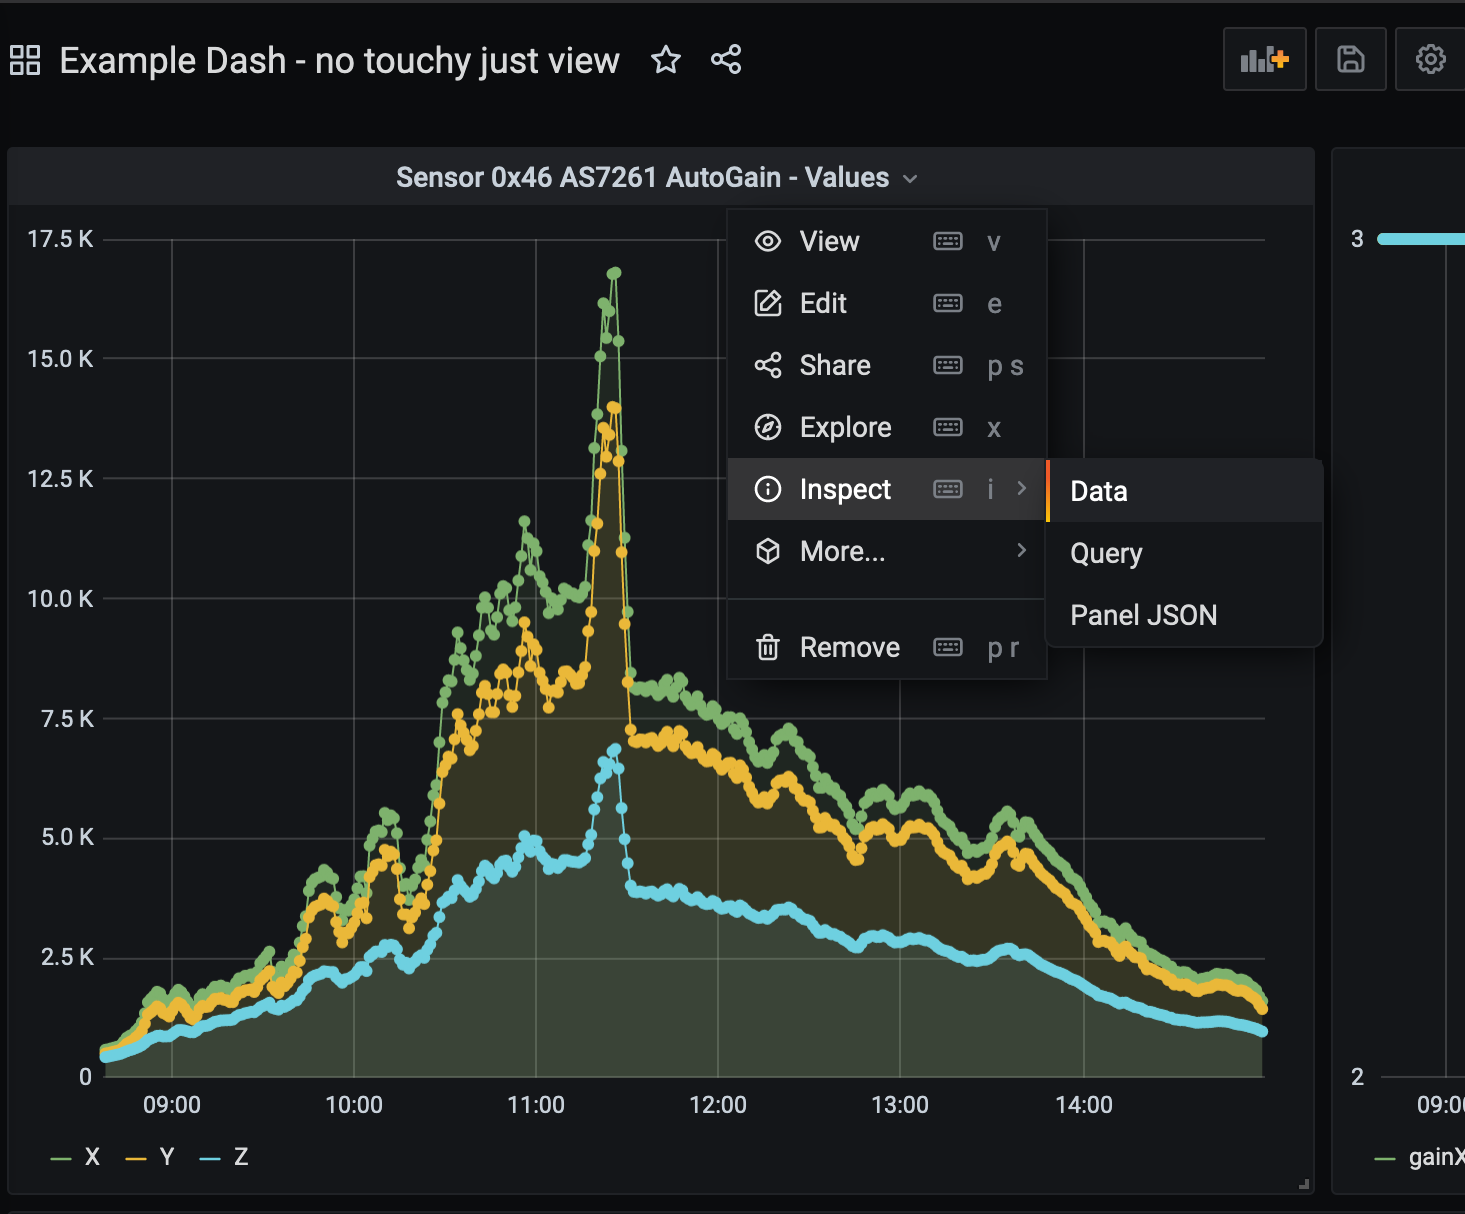
\includegraphics[width=0.6\textwidth]{img/handbuch/Export_Data}
\caption{Screenshot Grafana CSV-Export}
\label{fig:export_data}
\end{figure}
\noindent Daten können nur pro Plot exportiert werden. Um mehr Daten auf einmal zu exportieren, müssen alle gewünschten Daten in einem Plot vereint werden.

\subsection{Messsoftware Neustarten}
\label{restart}
Das Programm kann mit Control+C beendet werden.\\
Um es erneut zu starten sollte es neu kompiliert werden, da so immer alle eventuellen Einstellungsänderungen übernommen werden:\\
\textbf{sudo ~./SpectralSensor make}\\




\subsection{IP Adress Scan}
\paragraph{Unter Unix:} sudo nmap -sn 192.168.1.0/24  
\paragraph{Unter Windows:} Mit Hilfe der Software ''PortScan'' \\https://www.the-sz.com/products/portscan/\smallskip

\subsection{Bedeutung der Status LEDs}\label{leds}
\subsubsection{Rapsberry Pi}
Die rote PWR-LED leuchtet kontinuierlich bei stabiler 5 V Stromversorgung.\\
Die grüne ACT-LED blinkt, wenn die SD-Karte korrekt arbeitet.
\subsubsection{Status \& Adapterboard}
Die rote Power-LED zeigt an, dass die Messsoftware gestartet wurde.\\
Die grüne Heartbeat-LED ändert ihren Status nach jedem Messzyklus.\\


\subsection{Hilfe}
\textbf{Nach dem Starten der Messung gibt es keine Ausgabe in Terminal:}\\
Vermutlich sind keine Sensoren angeschlossen\\
\textbf{Die Systemzeit ist falsch:}\\
Keiner der NTP-Server aus der Liste /etc/systemd/timesyncd.conf kann erreicht werden.\\
\textbf{Das Webinterface ist nicht erreichbar:}\\
Entweder wurde die Adresse falsch geschrieben oder der Grafana-Server ist abgestürzt / wird nicht mehr automatisch gestartet.\\
\textbf{Error: 500
Write to Database Failed!:}
Der InfluxDB-Server ist abgestürzt / wird nicht mehr automatisch gestartet.
\subsection{Liste Der Verwendeten I2C Adressen \& Translationbytes}
\label{liste_Translationbytes}
Die Translation Bytes (Dezimal) 0- 59 wurden bereits verwendet. Sollten weitere Sensorboards angefertigt werden, muss es hier notiert werden:






